\documentclass[11pt]{article}
\usepackage[margin=1in]{geometry}
\usepackage{booktabs}
\usepackage{graphicx}
\usepackage{hyperref}
\usepackage{enumitem}
\setlist{itemsep=2pt,topsep=4pt}
\newcommand{\code}[1]{\texttt{#1}}

\title{A 10-iteration bounded check misses 1.3\% of wrong loop invariants\\
\large CSE 216, Team 10. Preliminary results, version 2}
\author{Working notes, 11 November 2026}
\date{}

\begin{document}
\maketitle

\noindent\textbf{AI-drafted notes.} Course policy requires the report text to be written by the
team. Every number comes from \code{src/analyze.py} in
\url{https://github.com/arelyx/invariant-grader-gap}.

\section*{Summary}

We graded 3{,}935 model-written loop invariants with a bounded model checker (ESBMC) and a full
verifier (UAutomizer). The Loop-R1 paper trains models with a bounded check at a bound under 10,
says it may accept false invariants, and gives no count.

\begin{center}
\begin{tabular}{rl}
\toprule
27 of 2{,}016 & wrong invariants accepted at a bound of 10 (1.3\%, 95\% interval 0.9--1.9) \\
4 of those 27 & are caused by the bound; the other 23 are a pointer-modelling difference \\
34 & invariants UAutomizer proved that are false when an \code{int} overflows \\
\bottomrule
\end{tabular}
\end{center}

\section{Finding 1 (most important): the tools disagree about C more than about the bound}

We expected one kind of disagreement: the bounded check accepts something that fails after
iteration 10. We found three, and that one is the smallest.

\begin{center}
\begin{tabular}{lrp{0.52\linewidth}}
\toprule
Kind & Candidates & Example \\
\midrule
Fails after the bound & 4 & \code{st == 0} on \code{nested\_delay\_notd2}. Accepted up to bound
20, rejected at 50. \\
Pointer compared with zero & 23 & \code{0 < head} on six linked-list programs. UAutomizer refutes
it. ESBMC accepts it at every bound it finishes, including 50. Cause not yet traced. \\
Signed overflow & 34 & Below. \\
\bottomrule
\end{tabular}
\end{center}

\noindent The overflow case, from \code{benchmark46\_disjunctive}:

\begin{verbatim}
int x, y, z;                         // arbitrary, at least one positive
while (nondet()) {
  assert(x > 0 || y > 0 || z > 0);   // candidate invariant
  if (x > 0) x++;
  if (y > 0) y++; else z++;
}
\end{verbatim}

\noindent UAutomizer proves it. ESBMC finds a failure on the second iteration:
\code{x = -1, y = -1, z = 2147483647}, then \code{z++} wraps to $-2147483648$. ESBMC treats
\code{int} as 32 bits. UAutomizer does not consider the wrapping run. With unbounded integers
(\code{--ir}) ESBMC agreed with UAutomizer on all three cases we re-ran.

Consequence for training: a model rewarded by UAutomizer learns invariants that break on 32-bit
hardware, and a model rewarded by ESBMC is penalised for invariants that hold over the
mathematical integers.

\section{Finding 2: the bound matters below 5 and not above}

\begin{center}
\begin{tabular}{rrr}
\toprule
bound & refuted invariants accepted (of 2{,}016) & true invariants timed out (of 1{,}628) \\
\midrule
1 & 737 (36.6\%) & 1.8\% \\
2 & 119 (5.9\%) & 2.8\% \\
5 & 27 (1.3\%) & 9.0\% \\
10 & 27 (1.3\%) & 12.8\% \\
20 & 26 (1.3\%) & 24.6\% \\
50 & 10 (0.5\%) & 41.7\% \\
\bottomrule
\end{tabular}
\end{center}

\noindent Wrong invariants from these models usually fail on iteration 1 or 2. Going from bound
10 to 50 catches 17 more and triples the timeouts.

\begin{center}
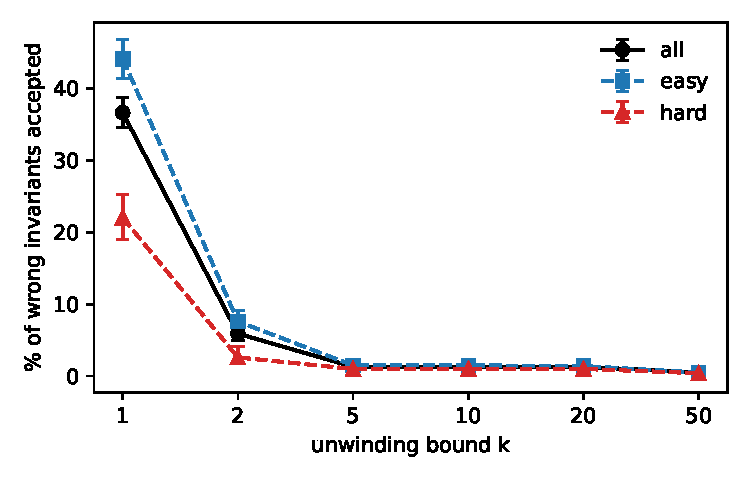
\includegraphics[width=0.55\linewidth]{../results/fig_bound_curve.pdf}
\end{center}

\section{Finding 3: the bounded check is a cheap way to choose among samples}

Eight samples per loop from Wonda's fine-tuned 4B model, 362 loops. Median time per check:
ESBMC 0.4\,s, UAutomizer 7.5\,s.

\begin{center}
\begin{tabular}{lr}
\toprule
Which sample is kept & Proved by UAutomizer \\
\midrule
The first one & 168/362 (46\%) \\
The first one ESBMC accepts at bound 10 & 253/362 (70\%) \\
Upper limit: any of the eight is provable & 277/362 (77\%) \\
\bottomrule
\end{tabular}
\end{center}

\section{What could overturn this}

\begin{enumerate}
\item \textbf{Short loops.} 103 of the 362 loops stop after a fixed small count, 26 of them
after one iteration. A bounded check cannot miss anything there. On long-running loops the
1.3\% could be much higher. This is the first thing to test.
\item \textbf{We guessed Loop-R1's setup.} Their code is unpublished. We used
\code{esbmc --unwind k --no-unwinding-assertions} from one sentence in the paper. Their reward
also has a Z3 check that we did not build.
\item \textbf{291 candidates have no verdict.} UAutomizer timed out. ESBMC accepted 109 of them
at bound 10, and any of those could be wrong.
\item \textbf{One model family.} All four models are Qwen3.
\item \textbf{Thin prior-work search.} We found no earlier count. We did not search exhaustively.
\end{enumerate}

\section{Setup}

\begin{center}
\begin{tabular}{lp{0.72\linewidth}}
\toprule
Programs & InvBench as shipped with Wonda: 219 C programs, 362 loops \\
Candidates & 1{,}086 from untrained Qwen3 0.6B, 1.7B and 4B, one per loop each. 2{,}896 from
Wonda's fine-tuned 4B, eight per loop. 3{,}935 parse as C. \\
What is checked & The program with \code{assert(candidate)} at the top of the loop body \\
Full verifier & UAutomizer, SV-COMP 2025. Limit 30\,s, or 120\,s on the 123 slow loops.
Result: 1{,}628 proved, 2{,}016 refuted, 291 no answer. \\
Bounded check & ESBMC 8.6 with \code{--32 --force-malloc-success} and pointer, bounds and
division checks off. Bounds 1, 2, 5, 10, 20, 50. Limit 30\,s. \\
\bottomrule
\end{tabular}
\end{center}

\noindent Two flags changed the numbers. Without \code{--force-malloc-success} ESBMC lets
\code{malloc} return \code{NULL} and rejects \code{x != NULL}, which UAutomizer proves. The
benchmark also uses \code{NULL} without a header, which ESBMC needs defined.

\section{Next three experiments}

\begin{enumerate}
\item Remove the iteration caps from the 103 capped programs and re-measure.
\item Run ESBMC with unbounded integers on everything, so overflow disagreements can be
subtracted out.
\item Find out why the tools disagree on \code{0 < head}.
\end{enumerate}

\section*{Sources}

Loop-R1 preprint, \url{https://www.ai2wj.com/data/Loop-R1-preprint.pdf}. Wonda,
arXiv:2603.15510. Quokka / InvBench, arXiv:2509.21629. ESBMC 8.6,
\url{https://github.com/esbmc/esbmc}. Ultimate Automizer, SV-COMP 2025 release.

\end{document}
